\chapter{Linearization} \label{Ch_Linerization}

A simple nonlinear system can be linearized in case it has simple relationships with $\sin$ or $\cos$ or $\tan$. For example the state of pendulums angular acceleration due to an input $u$ is expressed as:

\begin{equation} \label{Eq_Pendulum}
	\ddot{\theta} = -\frac{g}{l}\sin{\theta} + c u
\end{equation}

where, $c$ is a mapping coefficient that maps input torque $u$ to output accelerations $\ddot{\theta}$. Linearization is performed at defined points so called operating points (OP). In general, the OP are chosen such that the changes in the states of a system is zero. OP are local minima of a system, for example in a pendulum a local minima is when the pendulum is hanging straight down. Mathematically, this is defined as the path of the pendulum where the derivatives of the path are zero. Therefore, about OP $\theta_0$ when the pendulum is hanging straight down, the OP can be written as $(\theta_0,u_0)$. In the case of pendulum is hanging straight down, the input $u_0$ at this point is zero.

After having established this operating point, the conditions for which is completely known for us, any other state relative from this OP can be found. Theoretically, if any state $x$ is a relative distance $\delta x$ from $x_0$ and the inputs for which are at a relative distance $\delta u$ from the OP $u_0$, then it can be said that

\begin{equation} \label{Eq_Lin_OP1}
	(x_0,u_0) \rightarrow (x = x_0 + \delta x, u = u_0 + \delta u)
\end{equation}

For a nonlinear system such as one expressed by \eqref{Eq_Pendulum} written in the form:

\begin{equation}
	\dot{x} = f(x,u) \quad y = h(x)
\end{equation}

for the new deviations, the deviation dynamics can be written using equation \eqref{Eq_Lin_OP1}:

\begin{equation} \label{Eq_Lin_OP2}
	\dot{\delta} x = \frac{d}{dt}({x} + {x_0}) = \dot{x}
\end{equation}
where $\dot{x}_{0} = 0$ (because it is a constant OP) .The derivatives (evolution's) of these deviations becomes
\begin{equation} \label{Eq_Lin_OP3}
	\dot{\delta} x = \dot{x} = f(x_0 + \delta x, u_0 + \delta u)
\end{equation}
From equations \eqref{Eq_Lin_OP2} and \eqref{Eq_Lin_OP3}, it can be seen that the evolution of the states are same as the evolution of the deviations. Further, this evolution of the deviations as a function of the deviations and inputs when having a reference OP can be found using Taylor series expansion as given below
\begin{align} \label{Eq_Lin_OP4}
	\dot{\delta} x &= f(x_0 + \delta x, u_0 + \delta u) \\
	\dot{\delta} x &\approx f(x_0,u_0) + \frac{\partial f}{\partial x}(x_0,u_0) \delta x + \frac{\partial f}{\partial u}(x_0,u_0) \delta u \label{Eq_delta_x_delta_u} + \textbf{H.O.T}
\end{align}

Only the first two terms of Taylor's series are considered as they are only tangents to the actual deviations and also linear to the deviations. By considering such deviations to be linear to the actual deviations, the dynamics of the system now become linear. Although this assumption has reduced the dynamics to only the linear part, in real systems it has been found to produce excellent results (provided that Linearization is possible).

Similarly, the output deviation can be linearized as:

\begin{equation} \label{Eq_Lin_OP5}
	y = h(x_0,u_0) \approx h(x_0) + \frac{\partial h}{\partial x}(x_0,u_0) \delta x
\end{equation}

Additionally, in equations \eqref{Eq_Lin_OP4} and \eqref{Eq_Lin_OP5}, the OP are chosen such a way that their derivatives are zero (local minima or maxima). Therefore, the first terms from both these equations goes to zero, the remaining terms can be group into:
\begin{align} \label{Eq_Jacobians}
	\frac{\partial f}{\partial x}(x_0,u_0) &= \vec{A} \\
	\frac{\partial f}{\partial u}(x_0,u_0) &= \vec{B} \\
	\frac{\partial h}{\partial x}(x_0,u_0) &= \vec{C}
\end{align}

where, matrices $A,B,C$ are called \textbf{\textit{Jacobians}}, each of these terms are the elements of the matrices A, B and C.

Now from equations \eqref{Eq_Lin_OP4}, \eqref{Eq_Lin_OP5} and \eqref{Eq_Jacobians}, the state and output equations can be written as:
\begin{align}
	\dot{\delta} x &= \vec{A} \delta x + \vec{B} \delta u \\
	y &= \vec{C} \delta x
\end{align}
Therefore, the non-linear state equations are linearized using this method. Because the states in the linearized equation is $\delta x$ = $x - x_0$, and the input is $\delta u = u - u_0$ and output $\delta y = y - y_0$, the operating points have to be added and subtracted from the feedback system as shown in figure \ref{Fig_Lin_OP_FeedBack}
\begin{figure}[h!]
	\centering
	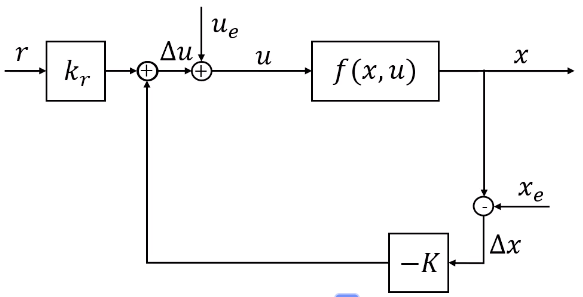
\includegraphics[width=0.65\linewidth]{Bilder/Lin_OP_FeedBack}
	\caption{Adding and subtracting OP's in feedback loop}
	\label{Fig_Lin_OP_FeedBack}
\end{figure}
\newpage

\section{Linearizing EoM of a pendulum}

Consider a pendulum with the state dynamics due to an input $u$ expressed by:

\begin{equation} \label{Eq_pendulum_Eom}
	\ddot{\theta} = -\frac{g}{l}\sin{\theta} + c u
\end{equation}

where, $c$ is the mapping factor that gives acceleration on $\theta$ coordinate for an input torque $u$. The term $\sin{\theta}$ makes the EoM \eqref{Eq_pendulum_Eom} nonlinear. Therefore, selecting an OP about $(\theta_0 = 0, u_0 = 0)$ from the position where the pendulum is hanging straight down. Also, consider the variable of state space as follows:

\begin{align*}
	x_1 &= \theta \\
	x_2 &= \dot{\theta}
\end{align*}

and output variable:

\begin{equation*}
	y = \theta
\end{equation*}

State dynamics can be written by the vector $\vec{\dot{x}}$ as:
\begin{equation} \label{Eq_f_pen_EoM}
	\vec{\dot{x}} = \begin{bmatrix}
		x_2 \\ \ddot{\theta}
	\end{bmatrix} = f(x, u) = \begin{bmatrix}
		x_2 \\ -\frac{g}{l}\sin{x_1} + c u
	\end{bmatrix}
\end{equation}
the output equation is just the state variable $x_1$:
\begin{equation}
	h(x) = x_1
\end{equation}
Jacobians are needs to determine matrices $\vec{A}$, $\vec{B}$ and $\vec{C}$ about the OP $(\theta_0,u_0)$ using \eqref{Eq_f_pen_EoM}:
\begin{equation*}
		\vec{A} = \begin{bmatrix}
			\frac{\partial f_1}{\partial x_1} & \frac{\partial f_1}{\partial x_2} \\
			\frac{\partial f_2}{\partial x_1} & \frac{\partial f_2}{\partial x_2}
		\end{bmatrix}_{(\theta_0,u_0)} = \begin{bmatrix}
			0 & 1 \\
			\frac{g}{l} \cos{x_1} & - u sin(x_1)
		\end{bmatrix}_{(0,0)}  = \begin{bmatrix}
			0 &1 \\ \frac{g}{l} & 0
			\end{bmatrix}
\end{equation*}
\begin{equation*}
\vec{B} = \begin{bmatrix}
\frac{\partial f_1}{\partial u_1} \\
\frac{\partial f_2}{\partial u_2}
\end{bmatrix}_{(\theta_0,u_0)} = \begin{bmatrix}
0 \\ cos(x_1)
\end{bmatrix}_{(0,0)}  = \begin{bmatrix}
0\\ 1
\end{bmatrix}
\end{equation*}
\begin{equation*}
\vec{C} = \begin{bmatrix}
1 & 0
\end{bmatrix}_{(\theta_0,u_0)} = \begin{bmatrix}
1 & 0
\end{bmatrix}_{(0,0)}  = \begin{bmatrix}
1 & 0
\end{bmatrix}
\end{equation*}

